\documentclass[tikz]{standalone}
\usepackage{tikz}
\usetikzlibrary{arrows.meta,positioning,fit,backgrounds}
\begin{document}
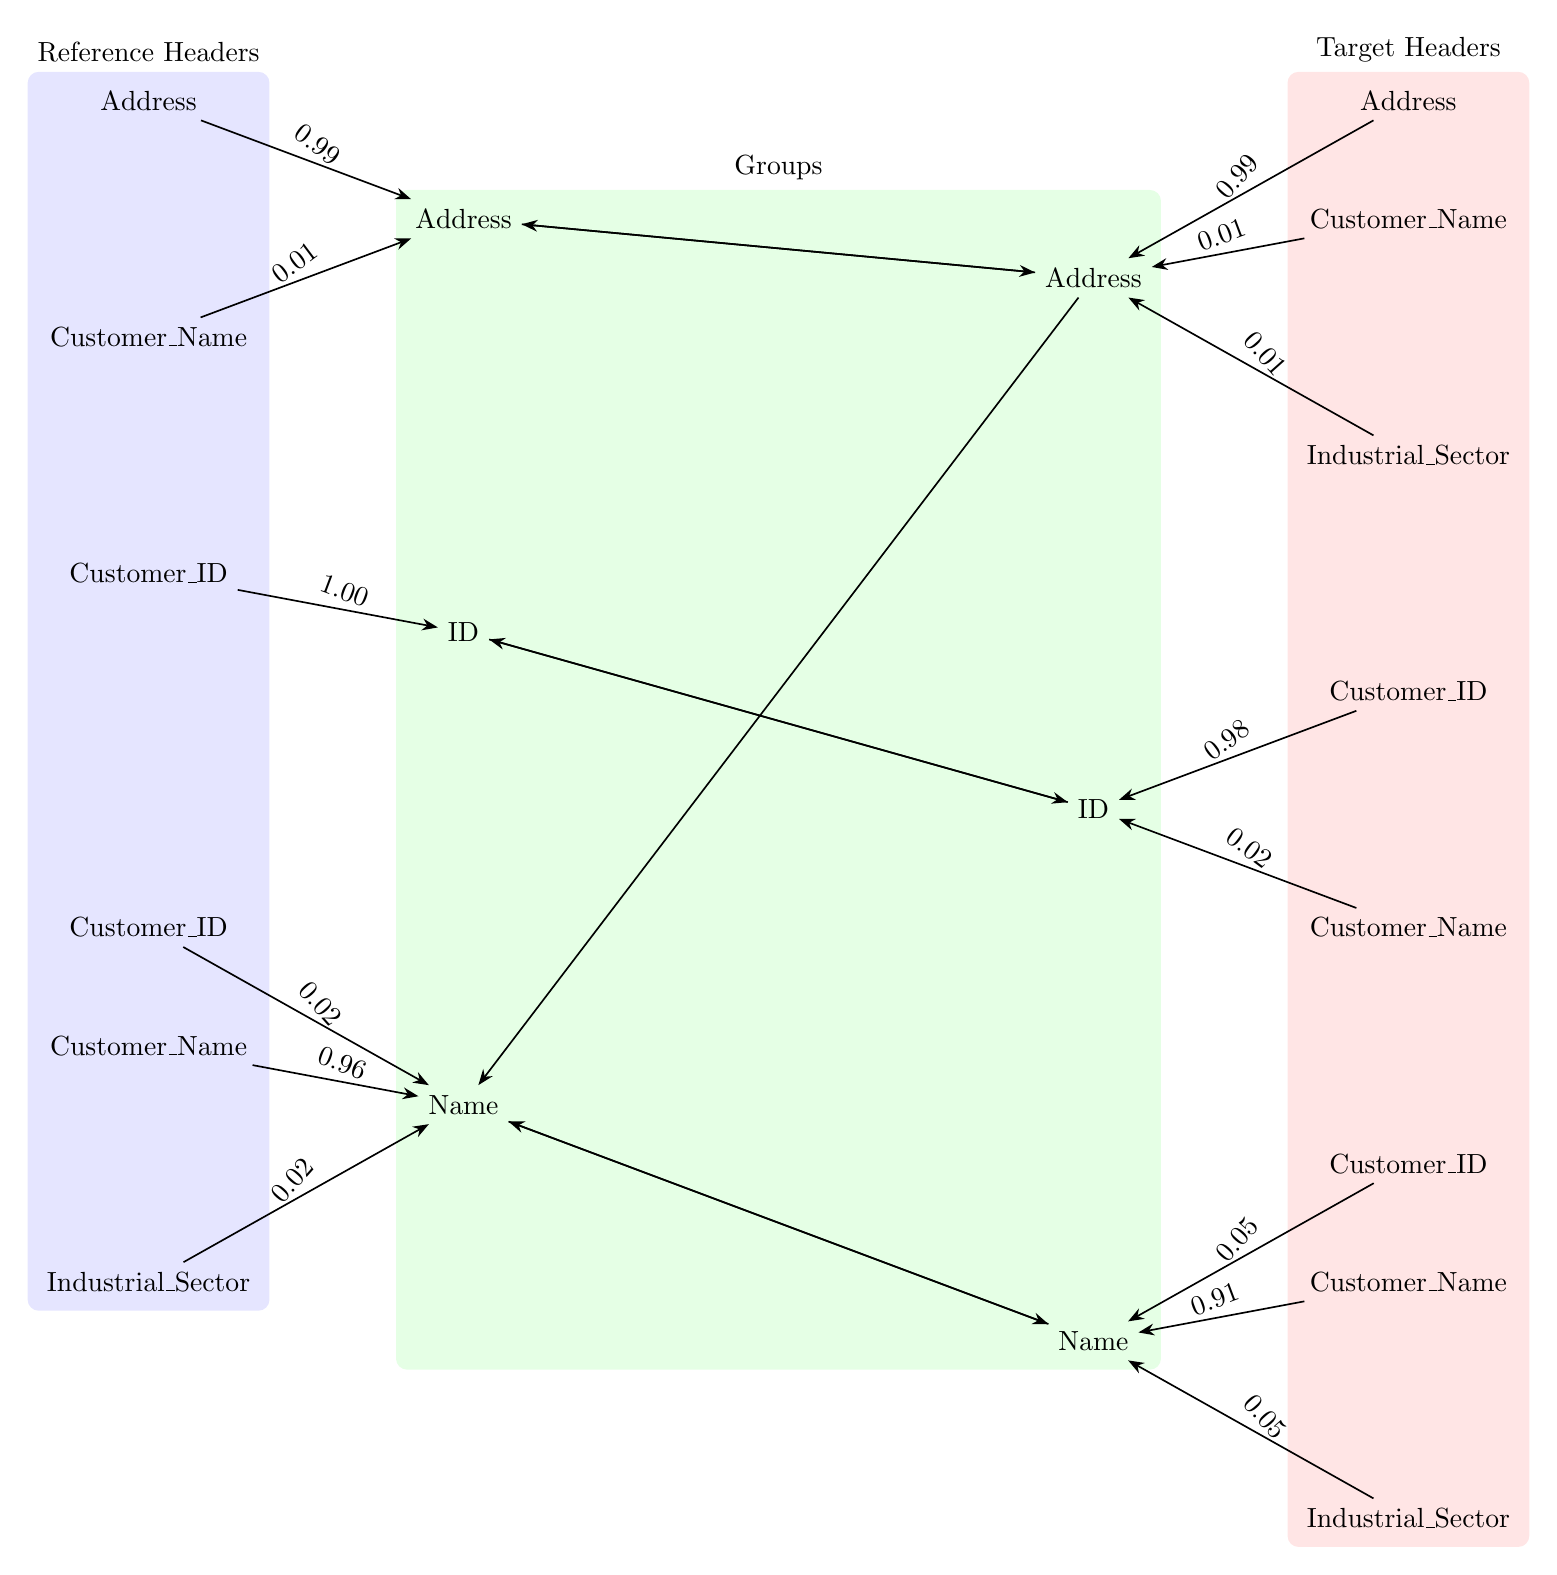
\begin{tikzpicture}[
    xscale=2,
    >={Stealth},
    auto,
    node distance=1.6cm,
    semithick
]

\node (refAddress) at (0.0, -1.50) {Address};
\node (hdrRefAddress_Address) at (-2.0, 0.00) {Address};
\draw[->] (hdrRefAddress_Address) -- node[midway,above,sloped,black]{0.99} (refAddress);
\node (hdrRefAddress_CustomerName) at (-2.0, -3.00) {Customer\_Name};
\draw[->] (hdrRefAddress_CustomerName) -- node[midway,above,sloped,black]{0.01} (refAddress);

\node (refID) at (0.0, -6.75) {ID};
\node (hdrRefID_CustomerID) at (-2.0, -6.00) {Customer\_ID};
\draw[->] (hdrRefID_CustomerID) -- node[midway,above,sloped,black]{1.00} (refID);

\node (refName) at (0.0, -12.75) {Name};
\node (hdrRefName_CustomerID) at (-2.0, -10.50) {Customer\_ID};
\draw[->] (hdrRefName_CustomerID) -- node[midway,above,sloped,black]{0.02} (refName);
\node (hdrRefName_CustomerName) at (-2.0, -12.00) {Customer\_Name};
\draw[->] (hdrRefName_CustomerName) -- node[midway,above,sloped,black]{0.96} (refName);
\node (hdrRefName_IndustrialSector) at (-2.0, -15.00) {Industrial\_Sector};
\draw[->] (hdrRefName_IndustrialSector) -- node[midway,above,sloped,black]{0.02} (refName);

\node (tgtAddress) at (4.0, -2.25) {Address};
\node (hdrTgtAddress_Address) at (6.0, 0.00) {Address};
\draw[->] (hdrTgtAddress_Address) -- node[midway,above,sloped,black]{0.99} (tgtAddress);
\node (hdrTgtAddress_CustomerName) at (6.0, -1.50) {Customer\_Name};
\draw[->] (hdrTgtAddress_CustomerName) -- node[midway,above,sloped,black]{0.01} (tgtAddress);
\node (hdrTgtAddress_IndustrialSector) at (6.0, -4.50) {Industrial\_Sector};
\draw[->] (hdrTgtAddress_IndustrialSector) -- node[midway,above,sloped,black]{0.01} (tgtAddress);

\node (tgtID) at (4.0, -9.00) {ID};
\node (hdrTgtID_CustomerID) at (6.0, -7.50) {Customer\_ID};
\draw[->] (hdrTgtID_CustomerID) -- node[midway,above,sloped,black]{0.98} (tgtID);
\node (hdrTgtID_CustomerName) at (6.0, -10.50) {Customer\_Name};
\draw[->] (hdrTgtID_CustomerName) -- node[midway,above,sloped,black]{0.02} (tgtID);

\node (tgtName) at (4.0, -15.75) {Name};
\node (hdrTgtName_CustomerID) at (6.0, -13.50) {Customer\_ID};
\draw[->] (hdrTgtName_CustomerID) -- node[midway,above,sloped,black]{0.05} (tgtName);
\node (hdrTgtName_CustomerName) at (6.0, -15.00) {Customer\_Name};
\draw[->] (hdrTgtName_CustomerName) -- node[midway,above,sloped,black]{0.91} (tgtName);
\node (hdrTgtName_IndustrialSector) at (6.0, -18.00) {Industrial\_Sector};
\draw[->] (hdrTgtName_IndustrialSector) -- node[midway,above,sloped,black]{0.05} (tgtName);


% -- Ref->Tgt edges --
\draw[->] (refAddress) -- (tgtAddress);
\draw[->] (refID) -- (tgtID);
\draw[->] (refName) -- (tgtName);

% -- Tgt->Ref edges --
\draw[->] (tgtAddress) -- (refAddress);
\draw[->] (tgtAddress) -- (refName);
\draw[->] (tgtID) -- (refID);
\draw[->] (tgtName) -- (refName);

% -- Background boxes for the three sections --
\begin{scope}[on background layer]
  \node[fill=blue!10,rounded corners,
        label=above:{Reference Headers},
        fit= (hdrRefAddress_Address)(hdrRefAddress_CustomerName)(hdrRefID_CustomerID)(hdrRefName_CustomerID)(hdrRefName_CustomerName)(hdrRefName_IndustrialSector)] {};
\end{scope}

\begin{scope}[on background layer]
  \node[fill=green!10,rounded corners,
        label=above:{Groups},
        fit= (refAddress)(refID)(refName)(tgtAddress)(tgtID)(tgtName)] {};
\end{scope}

\begin{scope}[on background layer]
  \node[fill=red!10,rounded corners,
        label=above:{Target Headers},
        fit= (hdrTgtAddress_Address)(hdrTgtAddress_CustomerName)(hdrTgtAddress_IndustrialSector)(hdrTgtID_CustomerID)(hdrTgtID_CustomerName)(hdrTgtName_CustomerID)(hdrTgtName_CustomerName)(hdrTgtName_IndustrialSector)] {};
\end{scope}

\end{tikzpicture}
\end{document}
